%!TEX root = <../index.tex>
\section{State of Art}
\label{sec:2}

In this section the concept, \textit{Semantic Text Similarity} (\textit{STS}), is introduced and several methods of similarity computation are reviewed. Section \ref{sec:2.1} interprets the concept \textit{STS}. The STS methods which are classified into two major categories are reviewed in section \ref{sec:2.2} and section \ref{sec:2.3} respectively. After that, we summarize in section \ref{sec:2.4} the commonly used technique of \textit{learning to rank}, which can be applied in our research from the viewpoint of \textit{information retrieval}. The section concludes with a formulation of the research questions. 

%The third part focuses on a short review of existent recommendation systems. 
\bigbreak
\subsection{Semantic Text Relatedness and Semantic Text Similarity}
\label{sec:2.1}

The objective of the thesis is to design a automatic system to discover related articles from the ZEIT corpus. However, ``related'' is not a well defined term. Nevertheless, if two articles are ``related'' to each other, they could be on the same topic or have other relationship like chronological relation. The methods of \textit{Semantic Textual Similarity} are able to compute the degree of such relationships. Before introducing the particular methods, we have to interpret what \textit{Semantic Text Similarity} is. We explain the concepts word by word. Starting with the last term of the concept, \textit{similarity} describes to what degree the characteristics of one object match the characteristics of another object. The second term \textit{textual} means a sequence of words with any length. The term \textit{document} is commonly mentioned as a synonym of \textit{text}. The term \textit{semantic} is the one of three levels of study of nature language including syntax, semantic and pragmatic. Semantics indicates that the concepts focuses on the literal and inherent meaning of nature language instead of the written or spoken form. In contrast, syntax is the study of the regularity of the combination of symbols without understanding their meaning in languages, and pragmatics studies how to understand the indeed intent of the speakers or authors. Semantics is in the middle of these three levels according to the complexity of understanding the real meaning of nature language. 

With combination of the three terms, \textit{Semantic Text Similarity} (STS) means how much the information of one text matches the information of another text. There is also a related concept: \textit{Semantic Relatedness}. However, the most researches on \textit{semantic relatedness} \citep{rohrbach2010helps, gracia2008web, gabrilovich2007computing} focus only on the relatedness between words or phrases but not on the texts. Therefore, it is an unrelated concept to our thesis. 

In our case, we define the similarity score between two documents is assigned from the closed interval $[0, 1]$. If the similarity degree between two texts is $1$, we say that these texts are absolutely similar. If the similarity degree is $0$, the texts are absolutely not similar. However, in some STS methods, the similarity degree can be negative and means that the texts have contrary meanings. Here an interesting open issue is whether one text is related to another text which has the contrary meanings. We use only non-negative value to indicate the similarity score.

There are many classification schemas to classify the existing methods. We introduce and assess three of them. 

\paragraph{Corpus-based and Knowledge-based}
The STS methods are usually categorized into two major classes, scilicet corpus-based and knowledge-based methods. Corpus-based methods try to compute the degree of similarity between texts using semantic information exclusively extracted from the large corpora. Normally, the corpora is used both in necessary knowledge generating (e.g. word2vec \cite{mikolov2013efficient}) and in model building. Meanwhile, the knowledge which is derived from other resources, e.g. Wikipedia, New York Times, is drawn into the initializing of models building in knowledge-based method. In our case, the corpus-based methods are preferred rather than knowledge-based methods. The reasons are briefly explained as follows. First, the existent knowledge-based measures are more suitable in the field of word similarity, e.g. \cite{jiang1997semantic}, \cite{strube2006wikirelate} and \cite{Agirre2009ta}, but they are relatively weak for dealing with documents or paragraphs. The second viewpoint is that the prior knowledge has less relevance to the target corpus. The importance and meaning of a word or phrase could be different in diverse sources, so that the knowledge from other sources could not interpret identical words in a specific corpus. Furthermore, the knowledge-based methods have unsatisfactory performance in case of dealing with the considerable number of Out of Vocabulary (OOV) words, whereas exactly compound words and inflection are ubiquitous in German. 

\paragraph{Compositional and Non-Compositional}

\cite{bar2013composite} proposes a classification schema which categorizes the STS methods into \textit{compositional methods} and \textit{non-compositional methods}. In short, \textit{compositional methods} treat a text as a sequence of words and compute the overall text similarity by aggregating pairwise word similarity. The representive methods are \citet{islam2008semantic} and \citet{tsatsaronis2010text}. \textit{Non-compositional methods}, e.g. \citet{gabrilovich2007computing} and \citet{kennedy2008evaluating}, regard a text as an entirety and represent it using a semantic model. The overall text similarity is computed by comparing the corresponding representations. 

\paragraph{String-based and Vector Space Model}

In the end, we propose a classification schema which categorize the STS methods into \textit{string-based methods} and \textit{vector space model (VSM) methods} according to the type of text representations and the approach of similarity computation. \textit{String-based methods} compute the text similarity through directly comparing the texts in string format and hence the complexity of similarity computation depends on the text length. \textit{VSM methods} represent a text as a vector with the fixed dimension and compute the text similarity through computing the relevance between the vectors. The similarity computation is only dependent on the dimension, whereas how to represent texts becomes the new issue. 
\bigbreak
\subsection{String-based Methods}
\label{sec:2.2}


\textit{String-based methods} have been used since several decades. The methods implement the naive idea that the texts are more similar if they share more same content. In the following parts, longest common subsequence, greedy string tiling and Jaccard coefficient based on the n-gram model are described respectively and their advantages and disadvantages are explained as well. 

\subsubsection{Longest Common Subsequence}

Given a string $s$, a subsequence of $s$ is any string in which the character is selected in $s$ with an arbitrary increasing order. The longest common subsequence of a set of strings is a string that is the maximal subsequence of all strings in the set. 

The longest common subsequence method treats one text as a sequence of characters and the text similarity is the ratio of the length of the longest common subsequence to the average length of the both texts. Mathematically, the similarity between two texts, $t_1$ and $t_2$, can be defined as: 

\begin{equation}
    sim_{LCS}(t_1, t_2) = 1 -  \frac{l(t_1) + l(t_2) - 2 \cdot l(lcs)}{l(t_1) + l(t_2)}
\end{equation}

where $lcs$ is the longest common subsequence of the texts and function $l$ is used for obtaining the length of a string. 

The method has drawbacks. One of them is that the measures do not utilize any semantics. Second, the method cannot use any sufficient optimization method, so that the operational efficiency is in a low level. According to \cite{paterson1994longest}, the time complexity of LCS is $O(mn)$ or a insignificant improvement with $O(n\cdot max(1, m/log n))$, where $m$ and $n$ are the length of the texts. Assumed there are $d$ documents in the corpus, $\overline{w}$ words for each document on average, and $\overline{c}$ characters for each word on average, the time complexity of LCS is $O(d \cdot (\overline{w} \cdot \overline{c})^2)$ for computing similarity between the target text and all rest texts in the corpus.

\subsubsection{Greedy String Tiling}

\cite{wise1993string} proposes Greedy String Tiling (GST) method. The purpose is to detect plagiarism in programming assignment of students. The algorithm works for two texts $t_1$ and $t_2$ as follows:
\begin{itemize}
    \item[1.] search the longest common substring of $t_1$ and $t_2$ which is also called the maximal match, and then remove the substring from $t_1$ and $t_2$.
    \item[2.] repeat the step 1, until the length of longest common substring is shorter than the pre-defined minimum match length.
    \item[3.] concatenate all obtained substrings as the common sequence ($gst$) of $t_1$ and $t_2$. 
\end{itemize}

Similar to LCS, the text similarity using GST is computed through the formula $1-\dfrac{l(t_1) + l(t_2) - 2 \cdot l(gst)}{l(t_1) + l(t_2)}$

In contrast with LCS, which is matched strictly ordered with texts, the result of GST is not strictly ordered, whereas it is enough that the maximal match in every iteration occurs in the texts exactly. GST is able to detect more common information of two texts, and it hence makes more sense for similarity computing than LCS. However, the time complexity is worse than LCS. It will be  $O(d \cdot (\overline{w} \cdot \overline{c})^3)$ in the worst case. Due to the high time complexity, this method is not used in the experiments.

Both of longest common subsequence and Greedy String Tiling regard texts as sequences of characters, so that they are not able to represent the latent relatedness of texts and they are no longer useful when they deal with long texts. Moreover, considering the operating efficiency these measures make sense only for short texts such as the titles of articles. 


\subsubsection{N-gram Models and Jaccard Similarity Coefficient}

An n-gram model is a commonly used model for analyzing the relation between an item and the former $n-1$ items and predicting the next item given the $n-1$ continuous items. The model is based on the assumption that the probability of occurrence of an item is only dependent on the combination of $n-1$ predecessors. An n-gram model with size $1$ is referred to as a ``unigram'', an model with size $2$ is a ``bigram'' and an model with size $3$ is a ``trigram''. Now we assume that all words in any text are selected from a set of words $\Sigma$ (or called vocabulary). From the viewpoint of n-gram, a text can be represented as a sequence of elements which are selected from the Cartesian product $\Sigma ^n$ of $\Sigma$ by $n$ times. N-gram models can work together with STS methods, so that the STS methods utilize not only the information of isolated words but also the information of the combination of several adjacent words. 

Jaccard similarity coefficient \citep{bank2008calculating} is a simple method for computing the similarity and diversity between two sets. For two texts $t_1=\{w^1_1, w^2_1, \cdots, w^{|t_1|-n+1}_1\}$, $t_2=\{w^1_2, w^2_2, \cdots, w^{|t_2|-n+1}_2\}$, where $w_i^j$ refers to the word at the $j$-th position in the text $i$. Jaccard similarity coefficient is defined as the size of the intersection divided by the size of the union. Formally,

\begin{equation}
    sim_{jaccard}(t_1, t_2) = \frac{|t_1 \cap t_2|}{|t_1 \cup t_2|} = \frac{|t_1 \cap t_2|}{|t_1| + |t_2| - |t_1 \cap t_2|}. 
\end{equation}

where $|t|$ is the number of distinct words in text $t$.

\bigbreak
\subsection{Vector Space Models}
\label{sec:2.3}

The idea of Vector Space Models (VSMs) is to represent a document as a vector in the vector space. The document is composed of a word sequence of an arbitrary or infinite (e.g. data streams) length, whereas the dimension of vector space is finite. Let $\mathbf{v}=(v_1, \cdots, v_n)$ represent a document $t$. Each dimension $v_i$ refers to a feature of the document. How to understand the $n$ features is defined differently according to the different hypothesis of the vector space. For example, each dimension corresponds the weight of a term in term-weighted vector spaces such Bag-of-Words and the weight of a topic in topic-weighted vector spaces, e.g. Latent Dirichlet Allocation. Once the dimension and the corresponding implication of the vector space are determined, each document is represented as a vector of the identical form, such that the text similarity can be transformed equivalently as computing the vector similarity. 

$cosine$ similarity of vectors is the most common used method. Let $\mathbf{v_1}=(v_1^1, \cdots, v_1^n)$ represent a document, $t_1$, and $\mathbf{v_2}=(v_2^1, \cdots, v_2^n)$ represent another document, $t_2$, $cosine$ similarity is defined as follows:

\begin{equation}
    sim_{cos}(t_1, t_2) = \frac{\mathbf{v_1} \cdot \mathbf{v_2}}{|\mathbf{v_1}| \cdot |\mathbf{v_2}|} = \frac{\sum_{i=1}^n v_1^i \cdot v_2^i}{\sqrt{\sum_{i=1}^n (v_1^i)^2} \cdot \sqrt{\sum_{i=1}^n (v_2^i)^2}}
\end{equation}

$cosine$ similarity of two documents ranges from 0 to 1, if the weight in each dimension is non-negative, for example, in term-weighted vector spaces. In some vector spaces such as Latent Semantic Index, the weight can be negative, such that the range of $cosine$ similarity is from -1 to 1. 

\textit{Pearson} product-moment correlation coefficient (PCC) is a measure of the linear correlation between two variables. Mathematically, PCC is defined in our case as: 

\begin{equation}
    sim_{PCC}(t_1, t_2) = \frac{(\mathbf{v_1-\overline{v}}) \cdot (\mathbf{v_2-\overline{v}})}{|\mathbf{v_1-\overline{v}}| \cdot |\mathbf{v_2}-\mathbf{\overline{v}}|} = \frac{\sum_{i=1}^n (v_1^i-\overline{v^i}) \cdot (v_2^i-\overline{v^i})}{\sqrt{\sum_{i=1}^n (v_1^i-\overline{v^i})^2} \cdot \sqrt{\sum_{i=1}^n (v_2^i-\overline{v^i})^2}}
\end{equation}
where $\mathbf{\overline{v}}=(\overline{v^1}, \cdots, \overline{v^n})$ is the expectation vector of all vectors which represent all documents in the corpus. An geometric interpretation of PCC is that the coordinate system is transformed by moving the coordinate origin to the vertex of the expectation vector and then the similarity between new vectors is computed. 

Another measure to indicate the similarity of vectors is to compute the distance of vectors, such as \textit{Euclidean} distance and \textit{Manhattan} distance. In this kind of similarity measure, vector normalization must be taken into account. One typical method is to make the norm of vectors as 1, such that the similarities between different vector pairs are comparable. For instance, \textit{Euclidean} distance is expressed as: 

\begin{equation}
    sim_{euclidean}(t_1, t_2) = 1 - \frac{|\mathbf{v_1 - v_2}|}{|\mathbf{v_{max} - v_{min}}|} = 1 - \frac{\sqrt{\sum_{i=1}^n (v_1^i-v_2^i)^2}}{\sqrt{\sum_{i=1}^n r^2}} ,
\end{equation}
where $r$ is the value range of every dimension and . 

\subsubsection{Bag-of-words and \tfidf{} Model}

Before defining the bag-of-words model, two concepts, ``word'' and ``term'', are interpreted. A ``word'' is the elementary unit of documents and a ``term'' is the unique element of a vocabulary which contains no duplicate words. 
In other words, we can say that the word at position $i$ of document $d$ is the word $w_t^i$, and that a term $t$ is used in document $d$ in $k$ times. 

The bag-of-words (BoW) model is a simple term-weighted vector space model. BoW discards the grammar and word order but only the occurrence frequency of terms remains. Each dimension of the vector space corresponds to the occurrence frequency of a term in the vocabulary and the size of dimension equals to the vocabulary size. The vocabulary can be either the universe set of terms which exist in the corpus or a subset of the universe, e.g. the most common $k$ terms or the terms being used at lease $k$ times. The BoW model has a crucial lack that some terms occur in the most documents frequently, such as ``go'', ``buy'' and ``play'' in English. After normalization, these common terms will occupy the dominating position and the weight of other terms will be insignificant. However, terms which occur infrequently in the entire corpus and repeatedly in specific clusters provide exactly more important semantic information. 

From this view point, term-frequency-inverse-document-frequency (\textit{tfidf}) exhibits the meaning or the characteristic of terms in the specific document instead of frequency itself of terms. The idea contains of two parts. On one side, the metric \textit{tf} indicates how frequent a term is in the target document. On the other side, the metric \textit{idf} refers to the scarcity of a term in the entire corpus. Given a document $d$ from the corpus $D$ and an arbitrary word $w_i$ in the vocabulary, 

\begin{equation}
    tfidf(w_i, d) = tf(w_i, d) \cdot log_2(\frac{|D|}{df(w_i, D)}), 
\end{equation}
where \textit{tf} is the number of occurrences of $w_i$ in $d$, and \textit{df} is the number of documents containing $w_i$. 

In both of BoW and \textit{tf-idf} models, there is a implicit assumption that the weight of a term is independent of its context and hence they are unable to cope with the complicate semantic analysis, such as polysemy, synonymy and the coexistence relation of terms. This shortcoming will be overcome in topic-weighted VSMs. Furthermore, disregarding the word order leads to lose semantic information, so that the critical idea of documents as well as the relationships like causality and temporal relationships are understood very difficultly. In the practical application, more than $90\%$ elements of vectors are zero, because the vocabulary size is usually much greater than the number of terms which are used in a single document. Due to the vector sparsity, the similarity computation will cost more time than expectation. 

\subsubsection{Latent Semantic Indexing}

In a BoW or \textit{tf-idf}  model, the features of a document are the weight of terms. However, the ideal features should describe the real idea of the author and the actual meaning of words. A word may have multiple meanings in different context. For example, ``apple'' is a kind of fruit in document about health, and is also a brand of smart-phone in documents about digital. Bow or \textit{tf-idf} can neither describe the differences of the identical term nor classify a containing the term document as the correct category. It is helpful to understand the exact meaning of words and of documents further, that the correlations between words in the corpus can be detected. The correlations is so-called latent semantic variables in the corpus, and one combination of correlations of all terms is called a ``topic''. The top $k$ topics are selected by ordering the importance of topics and then a document is represented accordingly as a vector in the latent semantic space where each dimension corresponds a selected topic. 

Latent Semantic Indexing applies Singular Value Decomposition (SVD) for decomposing the  $m\times n$ term-document matrix $N$. Let $N=TSD^t$, where $S$ is a $m\times n$ diagonal matrix, namely singular value matrix. The largest $k$ singular values are selected and the corresponding column vectors from $T$ and $D$ are also selected. At this moment, $S$ is approximated to a $k\times k$ matrix $\Sigma$, $T$ is approximated to a $k\times n$ matrix $U$ and $D$ is approximated to a $k\times m$ matrix $V$. As a result, the term-document matrix $N$ is the multiplication of three matrices approximately, scilicet $N=U\Sigma V^t$. The sketch of the process of LSI is depicted in figure \ref{fig:svd}.

\begin{figure}[!htb]
    \centering
    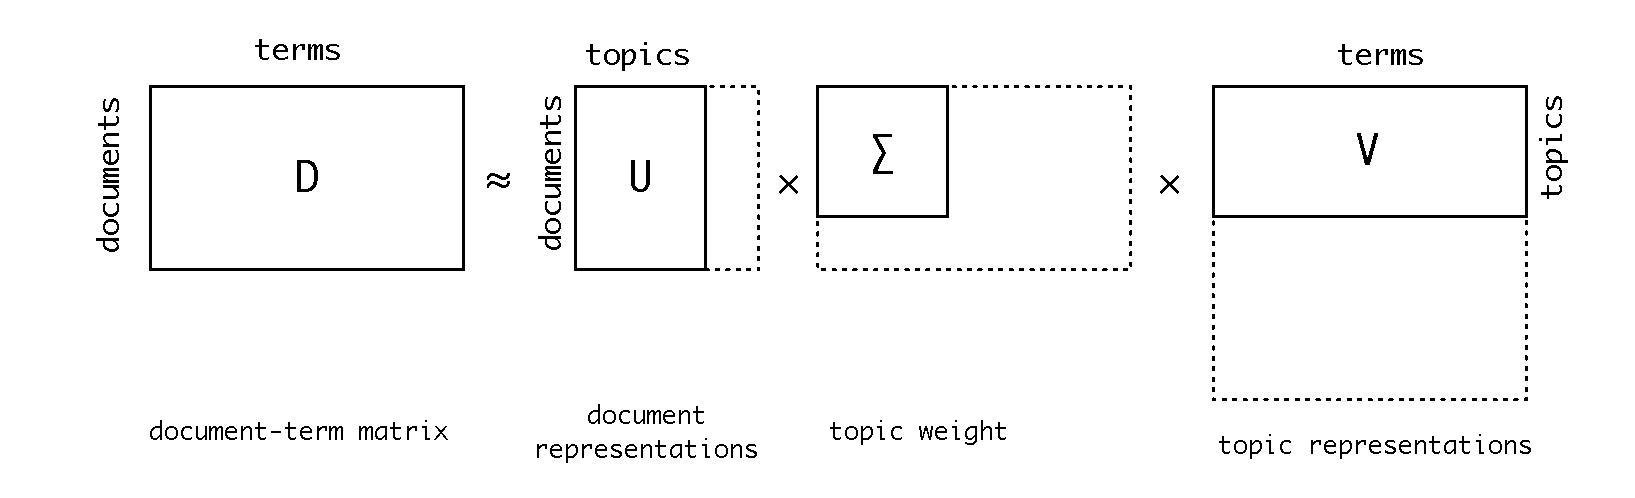
\includegraphics[width=1\textwidth]{fig/SVD.pdf}
    \caption[The sketch of the process of LSI using SVD]{the sketch of the process of LSI using SVD, where $D$ is the document-term matrix containing document representation of term weight, $U$ is the document-topic matrix containing document representations of topic weight, $\Sigma$ is the diagonal matrix containing the importance of topics and $V$ is the topic-term matrix containing the topic representations of term weight.}
    \label{fig:svd}
\end{figure}

After explaining the algorithm of LSI, we give the interpretation of every matrix. Each row vector of $U$ is the representation of the corresponding document in the latent semantic space of $k$-dimension. The representation refers to the topic distribution of the document. The row vectors of $V^t$ refers to the term distribution of the topics. The singular values in $\Sigma$ indicates the importance as well as the weight of the corresponding topics. 

The LSI model is able to recognize synonyms, which are represented as the similar vectors, and reduce the adverse impact of noise of data, so that the documents are profiled more precisely and more stably. However, it has also disadvantages. On the one hand, SVD is an operation with high complexity of runtime and memory. When a huge number of documents are trained or the model needs to update, the cost of SVD is probably intolerable (see section \ref{sec:5.3}). On the other hand, the model is not humanly readable. The representations of documents and topics cannot be interpreted directly according to their values. 

\subsubsection{Latent Dirichlet Allocation}

A Latent Dirichlet allocation model was presented as a probabilistic graphical model by \cite{Blei:2003}. LDA is a BoW-based topic model, which can compute the probability distribution of topics for a given document. Moreover, topics can be represented as a series of weighted words by LDA. 

The LDA model is a Bayesian generative model. From the view point of LDA, a document is generated in the following phases and the progress of generation is illustrated by figure \ref{fig:lda}.

\begin{itemize}
    \item[1.] select the topic distribution $\theta_i$ of the target document $d_i$ from the prior Dirichlet distribution $\alpha$, 
    \item[2.] generate a topic $z_{i,j}$ of $j$th word in the document $d_i$ from the multinomial topic distribution $\theta_i$ using Gibbs sampling,
    \item[3.] generate a word distribution $\Phi_{z_{i,j}}$ of the topic $z_{i,j}$ from the prior Dirichlet distribution $\beta$ using Gibbs sampling, 
    \item[4.] generate the word from the multinomial word distribution $\Phi_{z_{i,j}}$. 
\end{itemize}



\begin{figure}[!htb]
    \centering
    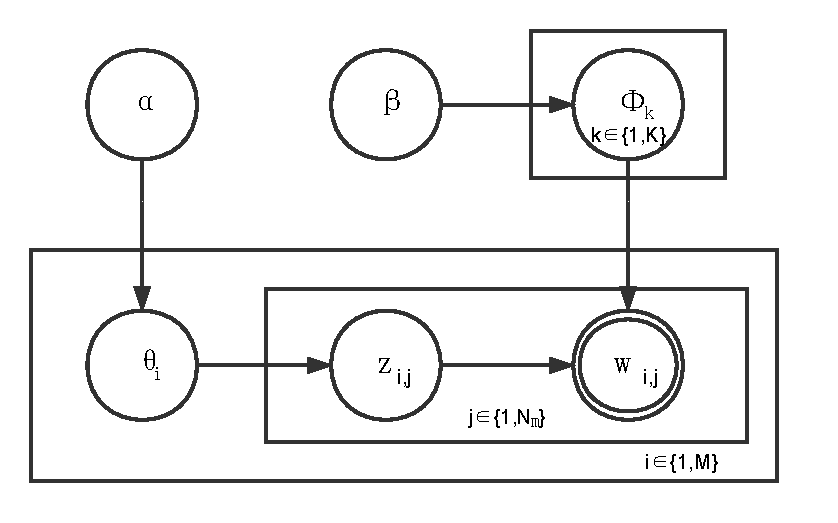
\includegraphics[width=0.5\textwidth]{fig/lda.pdf}
    \caption[Plate notation of representation of LDA]{Plate notation of representation of LDA. The dual-line plate refers to the observed variable, i.e. the posterior distribution of words in this case, and the monocoil plates indicate the latent variables, such as topic distribution and word distributions given a topic. The direction of arrows refer the conditional dependency of variables.}
    \label{fig:lda}
\end{figure}

The LDA model provides a general idea to build topic model. Since the work of \cite{Blei:2003}, subsequent research has explored many variant of LDA. There are four kinds of topic models so far, where are 1) unsupervised and non-hierarchical, 2) unsupervised and hierarchical, 3) supervised and non-hierarchical and 4) supervised and hierarchical. The main difference between supervised and unsupervised models is that each document has a response which could refers to the category or numeric rating. In the hierarchical approach, topics are organized hierarchically, in other words, one topic could have a super-topic and several sub-topics, such that document is understood more closely to the human understanding. The research and model names are drawn in the table \ref{tab:lda} respectively.
\begin{table}[!htb]
\centering
\resizebox{\textwidth}{!}{%
\begin{tabular}{|l|l|l|}
\hline
\textbf{Topic Models} & \textbf{non-hierarchical} & \textbf{hierarchical} \\ \hline
\textbf{unsupervised} & \begin{tabular}[c]{@{}l@{}}LDA, \cite{Blei:2003} \\ Correlated Topic Model, \cite{blei2006correlated} \end{tabular} & HLDA, \cite{sivic2008unsupervised} \\ \hline
\textbf{supervised} & \begin{tabular}[c]{@{}l@{}}sLDA, \cite{Blei:2008wy} \\ labeled LDA, \cite{ramage2009labeled} \end{tabular} & HSLDA, \cite{perotte2011hierarchically} \\ \hline
\end{tabular}%
}
\caption{Topic Model Variants of LDA}
\label{tab:lda}
\end{table}

\bigbreak

\subsection{Learning to Rank}
\label{sec:2.4}

The introduced in section \ref{sec:2.2} and \ref{sec:2.3} similarity methods extract the characteristics of documents and then compute the text similarity with unsupervised approaches. Learning to rank (LR) is an application of machine learning for document retrieval. The ranking function assigns the relevance degree for each candidate document in the corpus for a given query. The greater degree represents that the corresponding document is more relevant to the query. The documents are sorted in descending order of the corresponding relevance scores and then as the results of the retrieval. In the learning phase, a series of queries are provided and each query is associated with an ideal ordered list of documents. The LR model as well as the ranking function are trained using those lists of documents as training data. 

Due to the importance and necessity of ranking of the mass of relevant information, learning to rank is applied widely in search engine, recommendation systems and online advertising. According to the representation form of input data and the loss function, LR methods can be classified into three categories, namely pointwise, pairwise and listwise approaches \citet{liu2009learning}. 

We define the symbols which are mentioned in learning phase. $Q=(q^1,\cdots,q^m)$ denotes the collection of queries. A set of documents $d^i=(d_1^i, \cdots, d_{n^i}^i)$ is retrieved by the corresponding query $q^i$, where $n^i$ is the number of the related documents. $y_j^i$ denotes the true relevance degree of document $d_j^i$ to query $q^i$ and the degree is usually marked manually. $\mathbf{x}_j^i$ refers to the feature vector of the corresponding query-document pair. The key difference of strategies between pointwise, pairwise and listwise approaches is how to organize the query-document pairs as the training data and how to represent the predictions as output results. 

\paragraph{Pointwise Approach}

The pointwise approach is the most straightforward method to cope with the data. The pointwise approach does not process the feature vectors of query-document pair and applies the existing machine learning algorithms directly to compute the ranking. In this approach, the dependence of query and the comparison of the documents for the identical query are not taken into account. Quite a few common machine learning algorithms are suitable to apply in this approach. For example, polynomial regression \citep{fuhr1989optimum}, multi-class Vector Support Machines \citep{crammer2001algorithmic}, multi-class classification \citep{li2007mcrank} are the applications of the classic machine learning algorithms on the ranking. The pointwise approach have advantages. First, the existing algorithms are applied directly. Second, the number of training instance is minimal due to no additional data processing and the time cost for learning is quite satisfying. Nevertheless, that the query-level and the position information cannot be considered leads to the harm of performance.

\paragraph{Pairwise Approach}

The pairwise approach treats documents pair for the identical query as the training instance. In contrast with the pointwise approach, the results of ``preference'' function which make two feature vectors integrate for the same query, $\mathbf{x}_{u, v}^i = f(\mathbf{x}_u^i, \mathbf{x}_v^i)$, are used for the training instances in the pairwise approach. And the label $y_{u,v}^i$ of the new instances takes value from $\{+1, -1\}$. When $y_u^i$ is greater than $y_v^i$, $y_{u,v}^i$ equals $+1$, otherwise, $y_{u,v}^i$ is $-1$. The ranking problem is hence transformed to the classification problem. The varieties of the common classification models such as Vector Support Machines \citep{joachims2002optimizing}, Boosting \citep{freund2003efficient} and Neural Networks \citep{tsai2007frank} are applied. The ranking of the documents are generated from the relationship of the relevance degree between any documents pair. This approach offers shortcoming. First, the objective are partly different from the actual goal. In other words, the approach focuses on the optimizing the performance of classification of document pairs, whereas the actual goal is to find the optimal ranking of documents. Furthermore, the number of regenerated instances are too large. For query $q^i$, there are $\frac{n^i\cdot(n^i-1)}{2}$ instances as training data. 

\paragraph{Listwise Approach}

The listwise approach focuses on the real purpose of the ranking task and processes all retrieved documents for one query as an instance. Formally, an instance is represented as $\mathbf{x}^i = (\mathbf{x}_1^i, \cdots, \mathbf{x}_{n^i}^i)$. The label of instances have two forms according to the applied algorithms. One of them is the vector of relevance degree of all query-documents pair for a query, denoted as $y^i=(y_1^i, \cdots, y_{n^i}^i)$. The other form is the ranking of ordered documents, denoted as $y^i=(j_1^i, \cdots, j_{n}^i)$, where $n$ is the number of all documents and $y_{j_1^i}^i >= \cdots >= y_{j_n^i}^i$. The approach treats all feature vectors of documents as an entirety to train the model. In the first type of the algorithms (e.g. SoftRank \citep{taylor2008softrank} and SVM\textsuperscript{\textit{map}},  \citep{yu2005svm}), such as mean average precision (MAP) and normalized discounted cumulative gain (NDCG) are used as the evaluation measures for optimizing the models. In the second type of algorithms (e.g. ListNet \citep{cao2007learning}, ListMLE \citep{xia2008listwise}), the optimization methods focus on minimizing the inconsistency between the ranking prediction of the models and the true ranking of golden standard. 

The listwise approach uses all documents as the input data and the order of documents as the output label, so that the model is more impressive to deal with the differences between different queries. However, the complexity of the algorithms are higher than the other two approaches. 

\bigbreak

\subsection{Research Question}
\label{sec:2.5}

There is a nontrivial way from semantic text similarity to relatedness of documents. We attempt to find a systematic measure to discover related articles by one target article. The main task is to discover 2 candidates of related articles from the large corpora for a given target document automatically instead of manually. The most of researches have only discussed the degree of similarity between documents or the proportion of topics in each document and in the corpus. However, semantic text relatedness means means not only the semantic text similarity or the scale of a few common topics of documents. Four major questions have to be answered, so that achieving the relatedness degree of documents can be formulated more properly: 

\begin{description}
    \item[1.] \label{q:1} Can Semantic Text Similarity including string-based and vector space models methods be used to find related articles? How effective and efficient is the metrics of performance, such as precision and operational time?
    \item[2.] \label{q:2} How does the methods work in the practical scenario that the corpus keeps increasing with time? How is the performance of the incremental system different from a constant system? 
    \item[3.] \label{q:3} Is it useful to combine the STS methods? Does it yield to an improvement in performance or to a significant decrease of runtime?
    \item[4.] \label{q:4} The above introduced methods are unsupervised and ignore other meta-data. Does it lead to an improvement with utilizing supervised or semi-supervised algorithms which are proposed in the field of learning to rank?
\end{description}